\begin{explanationbox}
\begin{minipage}{\linewidth}
\textbf{位置一：小圆在椭圆内，仍然是 $r<d_{\min}$。}
取 $E:x^2/9+y^2/4=1$，圆心 $M=O$，半径 $r=1$。
圆心到椭圆的距离范围是 $[2,3]$。图中上下方向有最近间隙，
左右方向可取得最远距离。
% E: x^2/9+y^2/4=1; M=O; r=1; dmin=2, dmax=3.
\begin{center}
\begin{tikzpicture}[x=1cm,y=1cm,>=stealth,font=\small]
\draw[blue!70!black,thick] (0,0) ellipse (3 and 2);
\draw[orange!90!black,thick] (0,0) circle (1);
\draw[gray,dashed] (0,0)--(0,2);
\draw[red!75!black,very thick] (0,1)--(0,2);
\draw[<->,purple,thick] (-3,-2.7)--(1,-2.7) node[midway,below=4pt] {$D_{\max}=3+1=4$};
\draw[gray,dashed] (-3,0)--(-3,-2.9) (1,0)--(1,-2.9);
\fill (0,0) circle(2pt) node[below=5pt] {$M=O$};
\fill (0,1) circle(2pt);
\draw[gray] (-.1,1)--(-1.4,1.15) node[left=4pt,text=black] {$Q_1$};
\fill (0,2) circle(2pt) node[above=4pt] {$P_1$};
\fill (-3,0) circle(2pt) node[above left] {$P_2$};
\fill (1,0) circle(2pt) node[right=4pt] {$Q_2$};
\draw[red!75!black] (.1,1.5)--(1.2,2.7)--(3.4,2.7);
\node[red!75!black,anchor=west] at (3.6,2.7) {$D_{\min}=2-1=1$};
\node[blue!70!black] at (-2.9,1.7) {$E$};
\node[orange!90!black] at (-1.3,.8) {$\Gamma$};
\node[anchor=west,align=left] at (3.8,.5)
 {$r=1<d_{\min}=2$\\[5pt]圆周在椭圆内\\[5pt]两条边界仍有间隙};
\end{tikzpicture}
\end{center}

\end{minipage}
与首页的外离图比较：同样是 $r<d_{\min}$，圆周却在椭圆内部。
因此公式判断的是\textbf{两条边界间的距离}，不能单凭这个不等式判断圆在椭圆内还是外。
\end{explanationbox}

\begin{explanationbox}
\begin{minipage}{\linewidth}
\textbf{位置二：相交时，选同一个公共点，最近距离就是零。}
取 $E:x^2/4+y^2=1$，$\Gamma:(x-1)^2+y^2=4$。
此时 $d_{\min}=\sqrt{2/3}<r=2<d_{\max}=3$。
% E: x^2/4+y^2=1; Gamma: (x-1)^2+y^2=4.
% Intersections x=(4-2sqrt(10))/3; y=+-sqrt(1-x^2/4).
\begin{center}
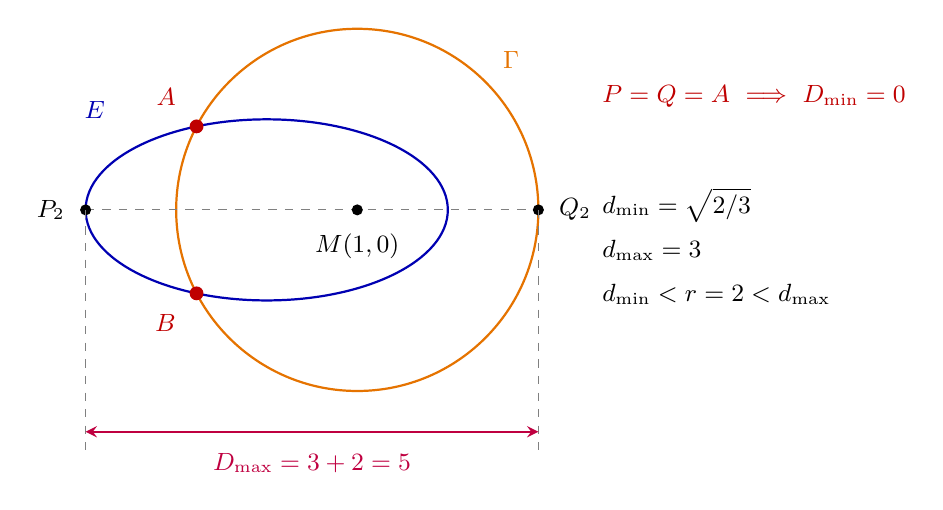
\begin{tikzpicture}[x=1.15cm,y=1.15cm,>=stealth,font=\small]
\pgfmathsetmacro{\ix}{(4-2*sqrt(10))/3}
\pgfmathsetmacro{\iy}{sqrt(1-\ix*\ix/4)}
\draw[blue!70!black,thick] (0,0) ellipse (2 and 1);
\draw[orange!90!black,thick] (1,0) circle (2);
\draw[gray,dashed] (-2,0)--(3,0);
\fill (1,0) circle(2pt) node[below=5pt] {$M(1,0)$};
\fill (-2,0) circle(2pt) node[left=4pt] {$P_2$};
\fill (3,0) circle(2pt) node[right=4pt] {$Q_2$};
\fill[red!75!black] (\ix,\iy) circle(2.5pt) node[above left=4pt] {$A$};
\fill[red!75!black] (\ix,-\iy) circle(2.5pt) node[below left=4pt] {$B$};
\node[red!75!black,anchor=west] at (3.6,1.25) {$P=Q=A\ \Longrightarrow\ D_{\min}=0$};
\node[blue!70!black] at (-1.9,1.1) {$E$};
\node[orange!90!black] at (2.7,1.65) {$\Gamma$};
\draw[gray,dashed] (-2,0)--(-2,-2.65) (3,0)--(3,-2.65);
\draw[<->,purple,thick] (-2,-2.45)--(3,-2.45)
 node[midway,below=4pt] {$D_{\max}=3+2=5$};
\node[anchor=west,align=left] at (3.6,-.4)
 {$d_{\min}=\sqrt{2/3}$\\[5pt]$d_{\max}=3$\\[5pt]$d_{\min}<r=2<d_{\max}$};
\end{tikzpicture}
\end{center}

\end{minipage}
图中 $A,B$ 均属于两条曲线；取 $P=Q=A$ 即得 $PQ=0$。
最远点仍需分别选取：$P_2(-2,0)$、$Q_2(3,0)$ 给出 $D_{\max}=5$。
\end{explanationbox}

\begin{explanationbox}
\begin{minipage}{\linewidth}
\textbf{位置三：等号边界也有公共点，不能遗漏相切。}
下图固定同一椭圆 $E:x^2/4+y^2=1$ 和圆心 $M=O$，只改变半径；
两幅图使用相同比例。左图半径取距离范围的下端点，右图取上端点。
% Same ellipse E: x^2/4+y^2=1, same centre M=O. Two endpoint radii.
\begin{center}
\begin{tikzpicture}[x=1.05cm,y=1.05cm,font=\small]
\begin{scope}
\node[font=\bfseries] at (0,3) {$r=d_{\min}=1$};
\draw[blue!70!black,thick] (0,0) ellipse (2 and 1);
\draw[orange!90!black,thick] (0,0) circle (1);
\fill (0,0) circle(2pt) node[right=4pt] {$M$};
\fill[red!75!black] (0,1) circle(2.5pt) node[above=5pt] {$A$};
\fill[red!75!black] (0,-1) circle(2.5pt) node[below=5pt] {$B$};
\node[align=center] at (0,-2.45) {圆在椭圆内，与椭圆相切\\[3pt]$D_{\min}=0$};
\end{scope}
\begin{scope}[xshift=7cm]
\node[font=\bfseries] at (0,3) {$r=d_{\max}=2$};
\draw[blue!70!black,thick] (0,0) ellipse (2 and 1);
\draw[orange!90!black,thick] (0,0) circle (2);
\fill (0,0) circle(2pt) node[right=4pt] {$M$};
\fill[red!75!black] (-2,0) circle(2.5pt) node[left=5pt] {$A$};
\fill[red!75!black] (2,0) circle(2.5pt) node[right=5pt] {$B$};
\node[align=center] at (0,-2.85) {圆包含椭圆，与椭圆相切\\[3pt]$D_{\min}=0$};
\end{scope}
\end{tikzpicture}
\end{center}

\end{minipage}
两种边界情形都有 $D_{\min}=0$。中间一段必须写成 $d_{\min}\le r\le d_{\max}$。
\end{explanationbox}

\begin{explanationbox}
\begin{minipage}{\linewidth}
\textbf{外切也是 $r=d_{\min}$ 的边界。}取同一椭圆，圆心移到 $M(4,0)$，半径取2。
% E: x^2/4+y^2=1; Gamma: (x-4)^2+y^2=4. External tangency at (2,0).
\begin{center}
\begin{tikzpicture}[x=1cm,y=1cm,font=\small,>=stealth]
\draw[blue!70!black,thick] (0,0) ellipse (2 and 1);
\draw[orange!90!black,thick] (4,0) circle(2);
\draw[gray,dashed] (-2,0)--(6,0);
\fill[red!75!black] (2,0) circle(2.5pt);
\draw[gray] (2,.1)--(2,1.5) node[above=5pt,text=red!75!black] {$A(2,0)$};
\fill (4,0) circle(2pt) node[below=5pt] {$M(4,0)$};
\fill (-2,0) circle(2pt) node[left=4pt] {$P_2$};
\fill (6,0) circle(2pt) node[right=4pt] {$Q_2$};
\node[blue!70!black] at (-1.8,1.3) {$E$};
\node[orange!90!black] at (5.6,1.65) {$\Gamma$};
\node at (1,2.9) {外切：$r=d_{\min}=2$，$D_{\min}=0$};
\draw[gray,dashed] (-2,0)--(-2,-2.8) (6,0)--(6,-2.8);
\draw[<->,purple,thick] (-2,-2.6)--(6,-2.6) node[midway,below=5pt] {$D_{\max}=6+2=8$};
\end{tikzpicture}
\end{center}

\end{minipage}
切点 $A$ 同时属于两条曲线，最近距离为零；最远点 $P_2(-2,0)$、$Q_2(6,0)$ 的距离为8。
\end{explanationbox}

\begin{explanationbox}
\begin{minipage}{\linewidth}
\textbf{位置四：圆包住椭圆时，最近距离反而要用最远圆心距离。}
下图取 $E:x^2/4+y^2=1$、$\Gamma:x^2+y^2=9$。每个椭圆点都在圆盘内，
离圆周最近的椭圆点，是离圆心最远的点，故 $D_{\min}=r-d_{\max}$。
% E: x^2/4+y^2=1; Gamma: x^2+y^2=9. dmax=2<r=3.
\begin{center}
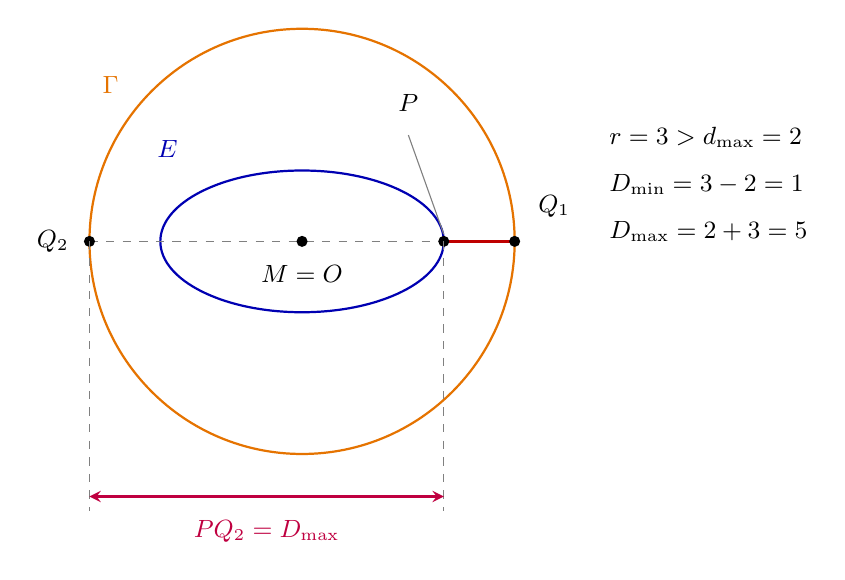
\begin{tikzpicture}[x=.9cm,y=.9cm,font=\small,>=stealth]
\draw[orange!90!black,thick] (0,0) circle(3);
\draw[blue!70!black,thick] (0,0) ellipse(2 and 1);
\draw[gray,dashed] (-3,0)--(3,0);
\draw[red!75!black,very thick] (2,0)--(3,0);
\fill (0,0) circle(2pt) node[below=5pt] {$M=O$};
\fill (2,0) circle(2pt);
\draw[gray] (2,.1)--(1.5,1.5) node[above=5pt,text=black] {$P$};
\fill (3,0) circle(2pt) node[above right=5pt] {$Q_1$};
\fill (-3,0) circle(2pt) node[left=4pt] {$Q_2$};
\node[blue!70!black] at (-1.9,1.3) {$E$};
\node[orange!90!black] at (-2.7,2.2) {$\Gamma$};
\node[anchor=west,align=left] at (4.2,.8)
 {$r=3>d_{\max}=2$\\[6pt]$D_{\min}=3-2=1$\\[6pt]$D_{\max}=2+3=5$};
\draw[gray,dashed] (-3,0)--(-3,-3.8) (2,0)--(2,-3.8);
\draw[<->,purple,thick] (-3,-3.6)--(2,-3.6) node[midway,below=5pt] {$PQ_2=D_{\max}$};
\end{tikzpicture}
\end{center}

\end{minipage}

\textbf{把图形判断压缩成数轴：}蓝段表示 $PM$ 的整个取值范围，
红点表示半径 $r$；最近距离就是红点到蓝段的距离。
% A distance to the closed interval, illustrated with numeric representative positions.
\begin{center}
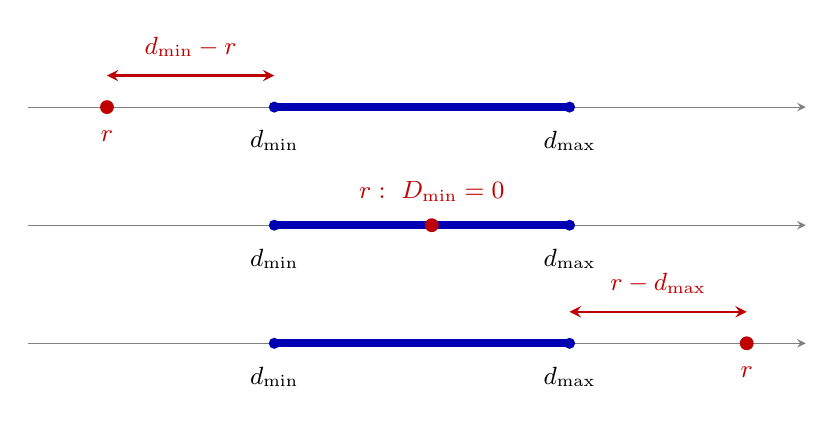
\begin{tikzpicture}[x=1.25cm,y=1cm,font=\small,>=stealth]
\foreach \yy in {0,-1.5,-3} {
 \draw[->,gray] (-.5,\yy)--(7.4,\yy);
 \draw[blue!70!black,line width=3pt] (2,\yy)--(5,\yy);
 \fill[blue!70!black] (2,\yy) circle(2pt) (5,\yy) circle(2pt);
 \node[below=5pt] at (2,\yy) {$d_{\min}$};
 \node[below=5pt] at (5,\yy) {$d_{\max}$};
}
\fill[red!75!black] (.3,0) circle(2.5pt) node[below=5pt] {$r$};
\draw[<->,red!75!black,thick] (.3,.4)--(2,.4) node[midway,above=3pt] {$d_{\min}-r$};
\fill[red!75!black] (3.6,-1.5) circle(2.5pt) node[above=5pt] {$r:\ D_{\min}=0$};
\fill[red!75!black] (6.8,-3) circle(2.5pt) node[below=5pt] {$r$};
\draw[<->,red!75!black,thick] (5,-2.6)--(6.8,-2.6) node[midway,above=3pt] {$r-d_{\max}$};
\end{tikzpicture}
\end{center}

红点落在蓝段上（含端点）时，存在 $PM=r$，即两条曲线有公共点。
红点在左侧取 $d_{\min}-r$，在右侧取 $r-d_{\max}$。
\end{explanationbox}
